\documentclass{article}
\usepackage[margin=1in,a4paper]{geometry}
\usepackage[utf8]{inputenc}
\usepackage{hyperref}
\usepackage{amsmath}
\usepackage{gensymb}
\usepackage{enumitem,amssymb}
\newlist{checks}{itemize}{2}
\setlist[checks]{label=$\square$}
\usepackage{graphicx}
\usepackage{amsthm}
\usepackage{amsfonts}
\usepackage{pdfpages}
\usepackage{pgfplots}
\pgfplotsset{compat=newest}
\usetikzlibrary{calc}
\usepackage{mathtools}
\usepackage{array}
\usepackage[T1]{fontenc}
\usepackage{lmodern}
\usepackage{tabularx}
\usepackage{fancyhdr}

\usepackage{xcolor}
\usepackage{nicefrac}
\usepackage{mdframed}
\usepackage[boxed,vlined]{algorithm2e}
\usepackage{cleveref}
% \usepackage{graphicx}
\newcommand{\Lim}[1]{\raisebox{0.0ex}{\scalebox{1}{$\displaystyle \lim_{#1}\;$}}}
\usepackage{graphicx}
\usepackage{tkz-tab}
\usepackage{fdsymbol}

\newcommand{\R}{\mathbb{R}}
\newcommand{\C}{\mathbb{C}}
\newcommand{\w}{\omega}
\newcommand{\p}{\partial}
\newcommand{\si}{&\quad\text{si }}
\DeclareMathOperator{\sinc}{sinc}
\DeclareMathOperator{\interior}{int}
\DeclareMathOperator{\adh}{adh}
\DeclareMathOperator{\argcosh}{argcosh}
\DeclareMathOperator{\argsinh}{argsinh}

\title{Exercices analyse}
\author{Dario Halilovic - Louis Martins Gonçalves - Aymeric - Tamara Paris}
\date{Septembre 2021}

\begin{document}

\maketitle

\section{Limites, suites et fonctions}
\subsection*{Exercice 1 ($\medblackstar \medwhitestar \medwhitestar$)}

Indiquez si les relations suivantes sont des fonctions ou non :
\begin{enumerate}
    \item $h(x) = \sin(x)$
    \item $\mathbb{Z} \to \mathbb{R}$\\
    $n \to \sqrt{\lvert n \rvert}$
    \item $x$ ayant pour image l'ensemble des $y$ tel que $x = y + 4$
    \item $a_n = \frac{n^2 + 2}{n^3 - 6n + 7}$ pour tout $n \in \mathbb{N}$
    \item $x$ ayant pour image l'ensemble des $y$ tel que $x = y^2$
    \item $f(x) = \left\{
    \begin{array}{ll}
        0 & \mbox{si } x \in \mathbb{Q}\\
        1 & \mbox{sinon}
        \end{array}
    \right.$
    \item $x$ ayant pour image $y$ comme sur ce graphique :\\
    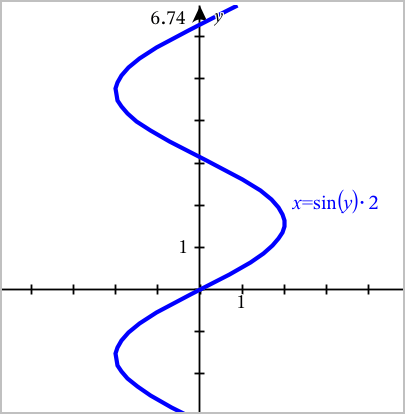
\includegraphics[width=7cm, height=6cm]{TextToGraph_2.png}
\end{enumerate}


\subsection*{Exercice 2 ($\medblackstar \medwhitestar \medwhitestar$)}

Trouver les limites des suites suivantes si elles existent lorsque $n$ tend vers $+\infty$ :

\begin{enumerate}
    \item $a_n = \frac{n^2 + 2}{7} + \frac{3}{n}$
    \item $a_n = \frac{7n^4 + 2}{4n^4}$
    \item $a_n = \frac{5n^2 + 2n + 1}{n^3 + 5}$
\end{enumerate}

\subsection*{Exercice 3 ($\medblackstar \medblackstar \medwhitestar$)}

Trouver les limites des suites suivantes si elles existent lorsque n tend vers $+\infty$ :

\begin{enumerate}
    \item $a_n = \cos(2n) + \frac{6}{n}$
    \item $a_n = \cos(2\pi n) + \frac{6}{n}$
    \item $a_n = \frac{\ln(e^n + n)}{n}$
    \item $a_n = \sqrt{n^2 + 4} - \sqrt{n^2 +n - 3}$
\end{enumerate}

\subsection*{Exercice 4 ($\medblackstar \medblackstar \medwhitestar$)}
\noindent Etudier les limites de fonctions suivantes :
\begin{enumerate}
    \item $\displaystyle\lim_{x \to 1^{+}}\ln(x)\ln(\ln(x))$
   
    
    \item $\displaystyle\lim_{x \to \frac{\pi}{2}}\frac{\sin(2x)}{\pi-2x}$\\
    (Hint : $\Lim{x \to 0} \frac{\sin(x)}{x} = 1$)
   
\end{enumerate}

\subsection*{Exercice 5 ($\medblackstar \medblackstar \medwhitestar$)}

Trouver des contre-exemple à ces affirmations (ça peut être simplement un schéma) :

\begin{itemize}
    \item Si la suite $b_n = cos(a_n)$ converge, alors la suite $(a_n)_{n \in \mathbb{N}}$ converge.
    \item Si la suite $b_n = \lvert a_n \rvert$ converge, alors la suite $(a_n)_{n \in \mathbb{N}}$ converge.
    \item Soient deux suites $(a_n)$ et $(b_n)$ tel que :
    \begin{itemize}
        \item $a_n \leq b_n$ pour $n$ pair
        \item $a_n \geq b_n$ pour $n$ impair
    \end{itemize}
    alors, si $(b_n)$ converge, $(a_n)$ converge aussi.
\end{itemize}
Remarque : Ces trois questions sont tombées en V/F en examen lors des années précédentes !

\subsection*{Exercice 6 ($\medblackstar \medblackstar \medblackstar$)}

\subsubsection*{Démonstration de l'unicité de la limite}

Nous allons démontrer pas à pas que la limite d'une fonction, si elle existe, est unique. Pour cela nous allons raisonner par "l'absurde", c'est à dire partir du principe qu'il peut exister plusieurs limite, et si nous arrivons à une contradiction, nous pouvons conclure qu'il ne peut pas en exister plusieurs.\\

\noindent Nous allons donc supposer qu'il existe une fonction $f$ telle que $\Lim{x \to a} f(x) = l$ et $\Lim{x \to a} f(x) = m$ avec $l \neq m$.\\

\noindent 1) Ecrivez les définitions mathématiques de $\Lim{x \to a} f(x) = l$ et de $\Lim{x \to a} f(x) = m$ avec $\epsilon$, $\delta_l$ et $\delta_m$.\\

\noindent 2) Exprimez $\delta$ en fonction de $\delta_l$ et $\delta_m$ afin que les définitions des deux limites exprimées dans le 1) soient encore correctes même lorsqu'on remplace $\delta_l$ et $\delta_m$ par $\delta$.\\

\noindent 3) Rappel (inégalité du triangle) : 
$$\lvert a + b \rvert \leq \lvert a \rvert + \lvert b \rvert $$

\noindent En prenant $\epsilon = \frac{\lvert l - m \rvert}{4}$, démontrer que $4\epsilon \leq \lvert l - f(x) \rvert + \lvert f(x) - m \rvert $.\\

\noindent 4) Démontrer à partir du résultat de la question précédente qu'on obtient $\epsilon \leq 0$ ce qui est une contradiction avec la définition de la limite (et donc que la limite d'une fonction est bien toujours unique).

\section{Continuité}

\subsection*{Exercice 1 ($\medblackstar \medwhitestar \medwhitestar$)}
\noindent Soit la fonction $g: \R \to \R$ définie de la manière suivante : \newline

$g(x)=\left \{
\begin{array}{rcl}
\frac{1}{\ln(\vert x \vert)} & \text{si} &x \not\in \{0,-1,1\} \\
0 &\text{sinon}&
\end{array}
\right.$
En quels points $g$ est-elle continue?
\subsection*{Exercice 2 ($\medblackstar \medblackstar \medwhitestar$)}%TVI
\noindent Soit $f:[0,1] \to [0,1]$ une fonction continue. L'affirmation suivante est-elle vraie ou fausse?\newline
$f$ admet toujours au moins un point fixe  
\footnote{On dit que $x$ est un point fixe de $f$ s'il vérifie $f(x)=x$}.\newline
(\textit{Hint}: Considérer la fonction $f(x)-x$. )

\subsection*{Exercice 3 ($\medblackstar \medblackstar \medwhitestar$)}
Sachant que $\sin(x) < x < \tan(x)$ pour tout $x$ tel que $0 < x < \frac{\pi}{2}$ comme il est illustré sur le schéma ci-dessous :\\
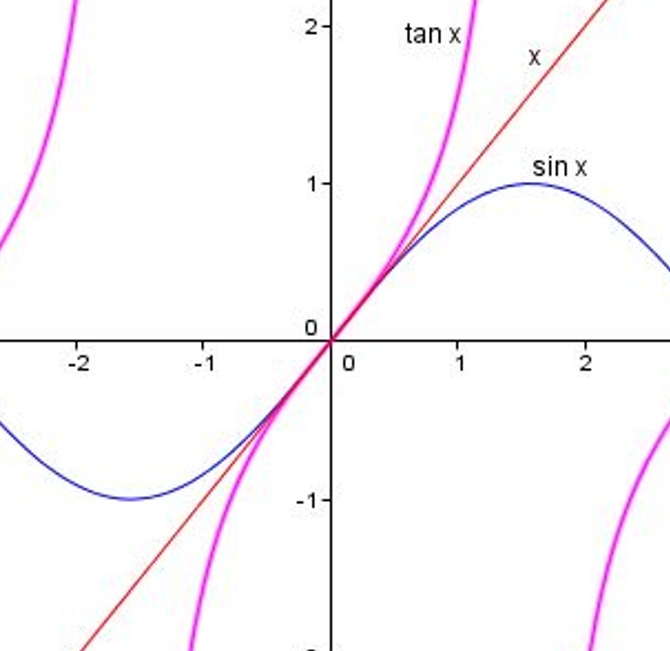
\includegraphics[width=7cm, height=6cm]{xsinxtanx.png}\\

\noindent La fonction $\displaystyle\frac{\sin(x)}{x}$ est-elle définie/continue en $0$? Dans le cas contraire, est-elle prolongeable par continuité en $0$?


\subsection*{Exercice 4 ($\medblackstar \medblackstar \medblackstar$, pour $\textbf{MA}$ et $\textbf{PH}$) }%TVI
\noindent Soit $f:\mathbb{R} \to \mathbb{R}$ continue telle que, pour tout $x \in \mathbb{R}$, on a $f(x)^{2}=1$. Démontrer que $f=1$ ou $f=-1$.

\section{Séries}
\subsection*{Exercice 1 ($\medblackstar \medwhitestar \medwhitestar$)}
Calculer les sommes suivantes :
\begin{enumerate}
    \item $\displaystyle\sum_{k=1}^{100} k$
    \item $\displaystyle\sum_{k=0}^{100} \frac{1}{2^{k}}$
    \item $\displaystyle\sum_{k=1}^{100} \frac{1}{k(k+1)}$

    \textit{Hint} : Etudier la différence $\frac{1}{k}-\frac{1}{k+1}$.

    \item $\displaystyle\sum_{k=2}^{100} \left(\frac{1}{\sqrt{k-1}}-\frac{1}{\sqrt{k}}\right)$
\end{enumerate}

\subsection*{Exercice 2 ($\medblackstar \medwhitestar \medwhitestar$)}
Expliquer pourquoi l'implication "série convergente implique absolument convergente" est fausse.\footnote{Une série convergente mais non absolument convergente est appelée \emph{semi-convergente}.}

\subsection*{Exercice 3 ($\medblackstar \medblackstar \medwhitestar$)}
\begin{enumerate}
    \item Démontrer par récurrence la formule des sommes partielles pour la série géométrique (avec $x \neq 1$)~:
    \[
    \sum_{k = 0}^{n} x^k = \frac{1 - x^{n+1}}{1 - x}
    \]
    \item En déduire la valeur de la série géométrique $\displaystyle\sum_{k = 0}^{\infty} x^k$ et son domaine de convergence (c'est-à-dire l'ensemble des valeurs de $x$ pour lesquelles la série converge).
\end{enumerate}

\subsection*{Exercice 4 ($\medblackstar \medblackstar \medwhitestar$)}
Utiliser le critère de comparaison pour déterminer la convergence ou divergence des séries suivantes :
\begin{enumerate}
    \item $\displaystyle\sum_{n = 1}^{\infty} \frac{1}{\sqrt[3]{n}}$
    \item $\displaystyle\sum_{n = 1}^{\infty} \frac{n(n-1)}{n^{\frac{8}{3}}}$
    \item $\displaystyle\sum_{n = 2}^{\infty} \frac{1}{n^2 \log(n)}$
    \item $\displaystyle\sum_{n = 1}^{\infty} \frac{a + (-1)^n}{n}$ pour $a > 1$
\end{enumerate}

\textit{Hint :} On rappelle que si $x \geq y > 0$ alors $\frac{1}{x} \leq \frac{1}{y}$.

\subsection*{Exercice 5 ($\medblackstar \medblackstar \medblackstar$)}
L'idée de cet exercice est de démontrer l'implication "convergence absolue implique convergence normale" pour les séries numériques (réelles).
\begin{enumerate}
    \item Soient $\displaystyle\sum_{n = 0}^{\infty} a_n = l \in \mathbb{R}$ et $\displaystyle\sum_{n = 0}^{\infty} b_n = q \in \mathbb{R}$ deux séries convergentes. Démontrer que la somme
    \[
    \sum_{n = 0}^{\infty} (a_n + b_n)
    \]
    converge.
    \item Soit $(a_n^+)$ une suite définie par $a_n^+ = a_n + |a_n|$. À titre d'exemple, on met ci-dessous quelques termes d'une suite quelconque $(a_n)$ et les termes correspondants pour $(a_n^+)$~:
    \begin{table}[h]
        \centering
        \begin{tabular}{|c|cccccc|}
        \hline
        $(a_n)$   & $2$ & $3$ & $-5$ & $6$  & $-2$ & \ldots \\
        \hline
        $(a_n^+)$ & $4$ & $6$ & $0$  & $12$ & $0$  & \ldots \\
        \hline
        \end{tabular}
        \label{tab:exo4}
    \end{table}
    
    Démontrer que si la série de terme $(a_n)$ converge absolument, la série $\displaystyle\sum_{n = 0}^{\infty} a_n^+$ est bornée et à termes positifs, donc convergente.
    \item En déduire en utilisant 1. que si $\displaystyle \sum_{n = 0}^{\infty} |a_n|$ converge, la série $\displaystyle \sum_{n = 0}^{\infty} a_n$ est convergente.
    
    \textit{Hint :} Exprimer $a_n$ en fonction de $a_n^+$ et $|a_n|$.
\end{enumerate}

\section{Nombres complexes}

\subsection*{Exercice 1 ($\medblackstar \medwhitestar \medwhitestar$)}

Pour les nombres complexes suivants, donnez leur partie réelle/imaginaire, leur module ainsi que leur augument, puis mettez-les sous leur forme polaire et exponentielle :
\begin{enumerate}
    \item $\sqrt{3}-i$
    \item $-4$
    \item $8i$
    \item $\dfrac{1-i}{i}$
\end{enumerate}

\subsection*{Exercice 2 ($\medblackstar \medblackstar \medwhitestar$)}

1) En passant par la forme exponentielle des nombres complexes, prouvez la formule de Moivre : $(\cos{\theta} + i\sin{\theta})^n= \cos{n\theta} + i\sin{n\theta}$ \\

\noindent 2) A partir de la formule de Moivre en déduire $\cos{2\theta}$ et $\sin{2\theta}$ en fonction de $\cos{\theta}$ et $\sin{\theta}$. \\

\noindent 3) On définit le conjugué d'un nombre complexe $z = x + iy$ par $\bar z = x - iy$. \begin{itemize}
    \item Donnez le conjugué des complexes suivant : $9+4i$, $i$, $4$
    \item Montrez que $z\bar z = |z|^2$.
    \item En visualisant le module et l'argument dans le plan complexe, donnez sans démontrer $|\bar z|$ et arg($\bar z$).
\end{itemize} 

\noindent 4) En se servant des questions précédentes, donnez la partie réelle et imaginaire des nombres complexes suivant : $\dfrac{1-i}{3+i}, (2-i)^8, \left(\dfrac{1}{i}\right)^{47}$ 

\subsection*{Exercice 3 ($\medblackstar \medblackstar \medwhitestar$)}

Sachant qu'on a que $(\pm i \sqrt{|\Delta|})^2 = -|\Delta|$, résolvez l'équation : 
\begin{equation*}
    z^2 -2z+2 = 0
\end{equation*}

\subsection*{Exercice 4 ($\medblackstar \medblackstar \medwhitestar$)}

Résolvez l'équation : $$z^2 = 1-i$$

\subsection*{Exercice 5 ($\medblackstar \medblackstar \medwhitestar$)}

Résolvez l'équation : $$z^6 = \sqrt{3} - i$$

\end{document}
